\section{扭转的概念}
\vspace*{-1.5em}
\begin{definition}[扭转变形]
	扭转变形是杆件受到大小相等,方向相反且作用平面垂直于杆件轴线的力偶作用,使杆件的横截面绕轴线产生转动。
	\begin{itemize}
		\item 受力特点
		\par 杆件的两端作用两个\md{大小相等}、\md{方向相反}、且\md{作用面垂直于杆件轴线}的力偶.
		\item 变形特点
		\par 杆件的任意两个横截面都发生绕轴线的相对转动.
	\end{itemize}
	\end{definition}

\section{外力偶矩的计算}
\vspace*{-1.5em}
\begin{theorem}[外力偶矩]
	工程中有许多传递功率的轴,需要根据它的转速$n$和传递的功率$N_p$计算出外力偶矩。力偶在单位时间内所作之功就是功率,它等于:
\begin{equation}
	N_p = M_n \omega
\end{equation}
$N_p$常用$\text{kw}$(千瓦)表示,而$w$常用$\text{rpm}$(转/分)表示.即
\margin{\\$M_\text{e}$ \quad 外力偶矩($\text{N}/\text{m}$)\\$P$ \quad 功率($\text{kw}$)\\$n$ \quad 转速($\text{r/min}$)}
\begin{equation}
	M_\text{e}=9549\,\frac{P}{n}
\end{equation}
\end{theorem}

\section{扭矩和扭矩图}
\subsection{扭矩的计算}

\smallboxa[截面法]{JMF} 求内力时,在$n-n$截面处假想将轴截开取左侧为研究对象,由
$$
\sum M_x = 0
$$
可以得到
\begin{equation}
	T=M_\text{e}
\end{equation}
其中$T$就称为\md{扭矩}.(参看图\ref{扭矩1}和图\ref{扭矩2})

\begin{figure}[!htbp]
	\centering
	
	\subfigure[扭转总体图]{
		\begin{minipage}[t]{0.5\linewidth}
			\centering
			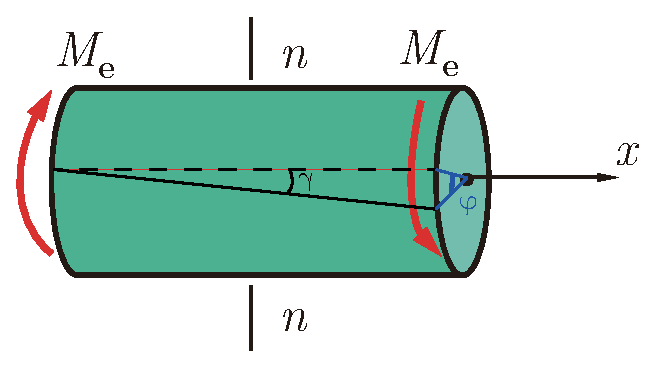
\includegraphics[width=0.9\linewidth]{picture/p2_c3/扭矩和扭矩图_1.eps}
			\label{扭矩1}
		\end{minipage}%
	}%
	\subfigure[扭矩图]{
		\begin{minipage}[t]{0.5\linewidth}
			\centering
			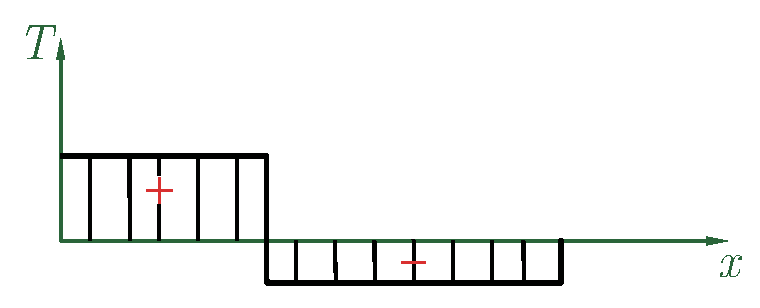
\includegraphics[width=0.9\linewidth]{picture/p2_c3/扭矩和扭矩图_4.eps}
			\label{扭矩4}
		\end{minipage}%
	}%

	%这个回车键很重要 \quad也可以
	\subfigure[截面左侧]{
		\begin{minipage}[t]{0.5\linewidth}
			\centering
			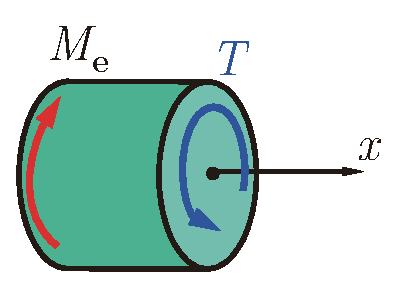
\includegraphics[width=0.7\linewidth]{picture/p2_c3/扭矩和扭矩图_2.eps}
			\label{扭矩2}
		\end{minipage}
	}%
	\subfigure[截面右侧]{
		\begin{minipage}[t]{0.5\linewidth}
			\centering
			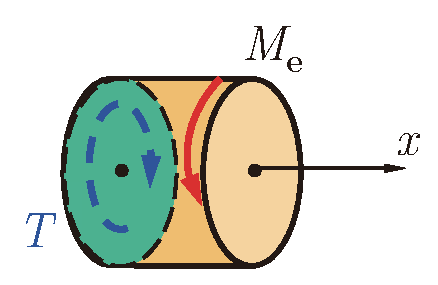
\includegraphics[width=0.75\linewidth]{picture/p2_c3/扭矩和扭矩图_3.eps}
			\label{扭矩3}
		\end{minipage}
	}%
	
	\centering
	\caption{扭矩与扭矩图}
\end{figure}

\subsection{扭矩的符号规定}
采用右手螺旋法则,当力偶矩矢的指向背离截面时扭矩为正,反之为负.

\subsection{扭矩图}
用平行于杆轴线的坐标 $x$ 表示横截面的位置;用垂直于杆轴线的坐标 $T$ 表示横截面上的扭矩,正的扭矩画在 $x$ 轴上方,负的扭矩画在 $x$轴下方.(参看图\ref{扭矩4})








